\header[v]{
    \section{De profundis morpionibus} \label{de-profundis-morpionibus}
    %
    
    \insertComment{Texte de Théophile Gautier (1864).}{}
}
\vspace{-0.7cm}
\enluminure{4}{\href{https://www.youtube.com/watch?v=YOvuIGmjckM}{O}}{h! muse} prête-moi ta lyre,
\\Afin qu'en vers je puisse dire
\\Un des combats les plus fameux,
\\Qui s'est déroulé sous les cieux.
\\\\\textbf{Refrain :}
\\De profundis morpionibus.
\\Et secatis roupettibus,
\\Et excita verolabus.
\\\\Dans un vagin de forte taille
\\600 000 poux livraient bataille
\\À un nombre égal de morpions
\\Qui défendaient l'entrée du con.
\\\\Le choc fut épouvantable
\\On croyait que c'était le diable
\\Les femm's enceintes en accouchant
\\Chiaient d'la merde au lieu d'enfants.
\bigskip
\begin{figure}[h!]
\centering
   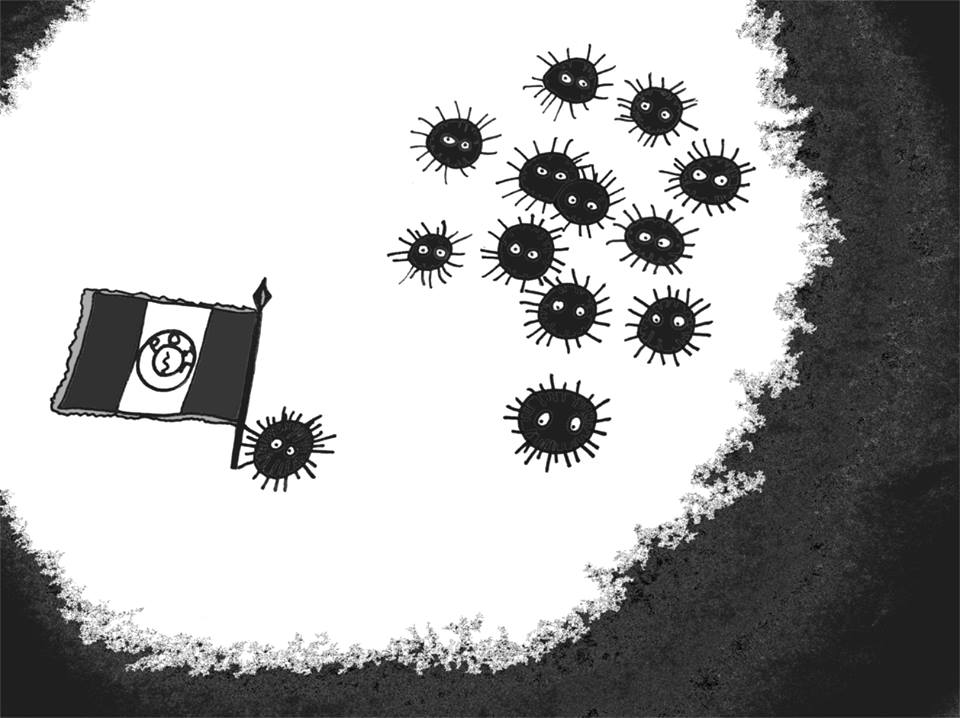
\includegraphics[width=0.7\textwidth]{images/de_profundis_morpionibus.jpg}
 \end{figure}
\breakpage
La bataille fut gigantesque
\\Tous les morpions périrent ou presque
\\À l'exception des plus trapus
\\Qui s'accrochaient aux poils du cul.
\\\\Ils ont bouché presque la fente
\\Que les morpions morts ensanglantent
\\Et la vallée du cul au con
\\Était jonchée de morpions.
\\\\Le commandant d'une escouade
\\Voyant périr ses camarades
\\Cria : Morpions ! Nous sommes foutus
\\Piquons un' charge au trou du cul.
\\\\Un morpion de noble origine
\\Qui revenait de Palestine
\\Leva sa lance et s'écria :
\\Les morpions meurent et n'se rendent pas.
\\\\Pour reprendre l'avantage
\\Les morpions luttaient avec rage
\\Mais leurs efforts furent superflus
\\Les poux gardèrent le dessus.
\\\\Le général nouvel Enée
\\Sortant des rangs de son armée
\\À son rival beau chevalier
\\Proposa un combat singulier.
\\\\À ch'val sur un poil de roupette
\\Armé d'une longue lorgnette
\\Le capitaine des morpions
\\Examinait les positions.
\\\\Tout à coup un obus arrive
\\Qui lui fait perdre l'équilibre
\\Le capitaine est bien foutu
\\Il tombe au fond du trou du cul.
\breakpage
\\\\Bardé d'un triple rang de crasse
\\Transpercé malgré sa cuirasse
\\Le capitaine des morpions
\\Tomba sans vie au fond du con.
\\\\Un morpion motocycliste
\\Prenant la raie du cul pour une piste
\\Vint avertir l'état-major
\\Que le capitaine était mort.
\\\\Pour retirer leur capitaine
\\Tous les morpions firent la chaîne
\\Mais hélas vains furent les efforts
\\L'abîme ne rend pas ses morts.
\\\\Puis au plus fort de la bataille
\\Soudain frappé par la mitraille
\\Le maréchal des morpions
\\Tomba mort à l'entrée du con.
\\\\Un soir au bord de la ravine
\\Tout couvert de foutre et d'urine
\\On vit un fantôme tout nu
\\À cheval sur un poil du cul.
\\\\C'était l'ombre du capitaine
\\De chancres et d'asticots pleine
\\Qui faute d'inhumation
\\Puait le maroilles et l'arpion.
\\\\Devant ce spectre qui murmure
\\D'être privé de sépulture
\\Tous les morpions firent serment
\\De lui él'ver un monument.
\\\\En vain l'on chercha sa dépouille
\\Sur la pine et sur les deux couilles
\\On ne trouva qu'un bout de queue
\\Qu'un sabre avait coupé en deux.
\breakpage
\\\\La troupe aussitôt prend les armes
\\L'enterre en versant force larmes
\\Comme au convoi d'un cardinal
\\Ou bien d'un garde national.
\\\\Puis les plus jolies morpionnes
\\Portaient en pleurant des couronnes
\\De fleurs blanch's et de poils de cul
\\Qu'avait tant aimé le vaincu.
\\\\Son cheval même l'accompagne
\\Et quatre morpions d'Espagne
\\Un' larme à l'œil le crêpe au bras
\\Tenaient les quatre coins du drap.
\\\\Au bord du profond précipice
\\On rangea les morpions novices
\\Ils déferlèr'nt par escadrons
\\Tout en sonnant de leurs clairons.
\\\\Ils le suivirent au cimetière
\\S'assirent en rond sur leur derrière
\\La crotte au cul, la larme à l'œil
\\Tous les morpions étaient en deuil.
\\\\On lui él'va un cénotaphe
\\Où l'on grava cette épitaphe
\\"Ci-gît un morpion de valeur
\\Tombé sans vie au champ d'honneur."
\\\\Et l'on en fit une relique
\\Que l'on mit dans un' basilique
\\Pour que les futurs bataillons
\\Sachent comment meurt un morpion.
\\\\Sur une couill' grosse et velue
\\L'on érigea une statue
\\À ce capitain' de morpions
\\Mort si brav'ment au fond d'un con.
\breakpage
\\\\Depuis ce jour on voit dans l'ombre
\\À la porte d'un caveau sombre
\\Les morpions de noir vêtus
\\Montant la garde au trou du cul.
\\\\Depuis ce temps dans la vallée
\\On entend des bruits de mêlée
\\Les morpions pour venger l'vaincu
\\S'cramponnent à tous les poils du cul.
\\\\Et parfois les soirs de brume
\\Quand sur la terr' se lèv' la lune
\\On voit les âmes des morpions
\\Voltiger sur les poils du con.
\\
\begin{figure}[h!]
\centering
   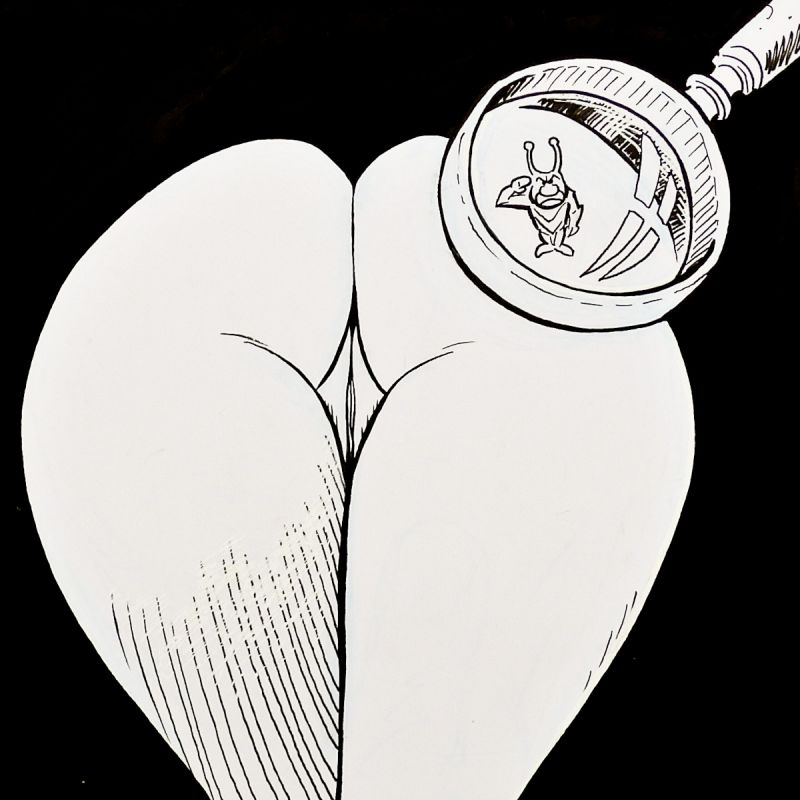
\includegraphics[width=0.9\textwidth]{images/de_profondis.jpg}
 \end{figure}

\breakpage